
\serie{Composantes d'un vecteur}

\begin{exercice}
On se place dans un repère $(O;\vec{i};\vec{j})$.\\ Soient $A(-1;3)$, $B(2;5)$, $C(2;-2)$ et $D(1;0)$.
Déterminer les composantes des vecteurs $\overrightarrow{AB}$, $\overrightarrow{AC}$, $\overrightarrow{BD}$, $\overrightarrow{AC}+\overrightarrow{BD}$, $\overrightarrow{DA}$, $\overrightarrow{BA}$ et $\overrightarrow{DC}+\overrightarrow{AB}$.
\end{exercice}

\begin{exercice}
On se place dans un repère $(O;\vec{i};\vec{j})$
\begin{center}
\definecolor{qqqqff}{rgb}{0,0,1}
\definecolor{cqcqcq}{rgb}{0.75,0.75,0.75}
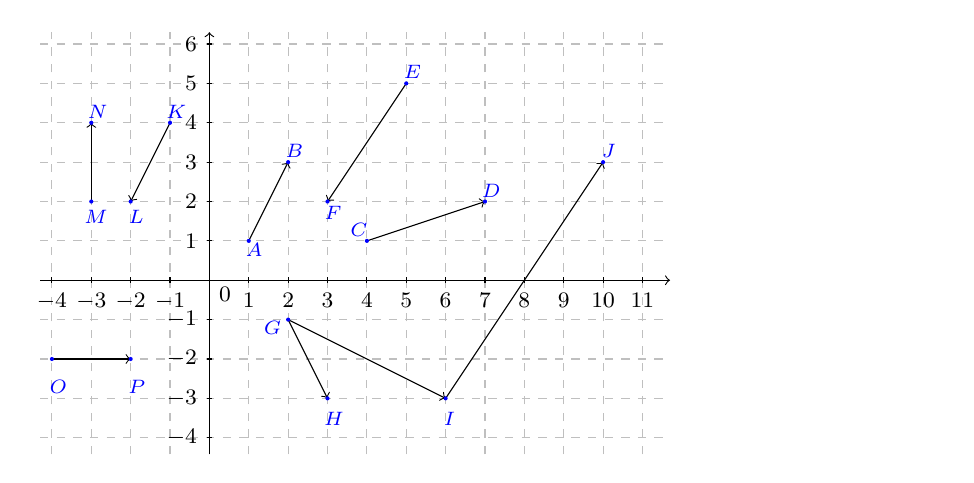
\begin{tikzpicture}[scale=0.5][line cap=round,line join=round,>=triangle 45,x=1.0cm,y=1.0cm]
\draw [color=cqcqcq,dash pattern=on 3pt off 3pt, xstep=1.0cm,ystep=1.0cm] (-4.3,-4.42) grid (11.7,6.3);
\draw[->,color=black] (-4.3,0) -- (11.7,0);
\foreach \x in {-4,-3,-2,-1,1,2,3,4,5,6,7,8,9,10,11}
\draw[shift={(\x,0)},color=black] (0pt,2pt) -- (0pt,-2pt) node[below] {\footnotesize $\x$};
\draw[->,color=black] (0,-4.42) -- (0,6.3);
\foreach \y in {-4,-3,-2,-1,1,2,3,4,5,6}
\draw[shift={(0,\y)},color=black] (2pt,0pt) -- (-2pt,0pt) node[left] {\footnotesize $\y$};
\draw[color=black] (0pt,-10pt) node[right] {\footnotesize $0$};
\clip(-4.3,-4.42) rectangle (18.7,6.3);
\draw [->] (1,1) -- (2,3);
\draw [->] (4,1) -- (7,2);
\draw [->] (5,5) -- (3,2);
\draw [->] (2,-1) -- (3,-3);
\draw [->] (6,-3) -- (10,3);
\draw [->] (-1,4) -- (-2,2);
\draw [->] (-3,2) -- (-3,4);
\draw [->] (-4,-2) -- (-2,-2);
\draw [->] (2,-1) -- (6,-3);
\begin{scriptsize}
\fill [color=qqqqff] (1,1) circle (1.5pt);
\draw[color=qqqqff] (1.14,0.78) node {$A$};
\fill [color=qqqqff] (2,3) circle (1.5pt);
\draw[color=qqqqff] (2.16,3.28) node {$B$};
\fill [color=qqqqff] (4,1) circle (1.5pt);
\draw[color=qqqqff] (3.8,1.28) node {$C$};
\fill [color=qqqqff] (7,2) circle (1.5pt);
\draw[color=qqqqff] (7.16,2.28) node {$D$};
\fill [color=qqqqff] (5,5) circle (1.5pt);
\draw[color=qqqqff] (5.16,5.28) node {$E$};
\fill [color=qqqqff] (3,2) circle (1.5pt);
\draw[color=qqqqff] (3.14,1.7) node {$F$};
\fill [color=qqqqff] (2,-1) circle (1.5pt);
\draw[color=qqqqff] (1.6,-1.2) node {$G$};
\fill [color=qqqqff] (3,-3) circle (1.5pt);
\draw[color=qqqqff] (3.16,-3.52) node {$H$};
\fill [color=qqqqff] (6,-3) circle (1.5pt);
\draw[color=qqqqff] (6.1,-3.52) node {$I$};
\fill [color=qqqqff] (10,3) circle (1.5pt);
\draw[color=qqqqff] (10.14,3.28) node {$J$};
\fill [color=qqqqff] (-1,4) circle (1.5pt);
\draw[color=qqqqff] (-0.84,4.28) node {$K$};
\fill [color=qqqqff] (-2,2) circle (1.5pt);
\draw[color=qqqqff] (-1.86,1.6) node {$L$};
\fill [color=qqqqff] (-3,2) circle (1.5pt);
\draw[color=qqqqff] (-2.88,1.6) node {$M$};
\fill [color=qqqqff] (-3,4) circle (1.5pt);
\draw[color=qqqqff] (-2.84,4.28) node {$N$};
\fill [color=qqqqff] (-4,-2) circle (1.5pt);
\draw[color=qqqqff] (-3.84,-2.72) node {$O$};
\fill [color=qqqqff] (-2,-2) circle (1.5pt);
\draw[color=qqqqff] (-1.84,-2.72) node {$P$};
\end{scriptsize}
\end{tikzpicture}
\end{center}
Déterminer les composantes des vecteurs représentés sur le graphique.
\end{exercice}

\begin{exercice}
On se place dans un repère $(O;\vec{i};\vec{j})$.\\ 
Soit $A(2;-1)$, $B(-1;3)$, $C(-2;-2)$ et $D(-5;2)$.
Déterminer les composantes de $\overrightarrow{DB}$ et $\overrightarrow{CA}$. 

Que peut-on dire du quadrilatère $ABDC$?
\end{exercice}

\begin{exercice}
On se place dans un repère $(O;\vec{i};\vec{j})$.\\ 
Soient $A(-1;-1)$, $B(2;5)$ et $C(2;0)$. 

Déterminer les coordonnées de $D(x;y)$ pour que $\overrightarrow{AB}=\overrightarrow{DC}$.
\end{exercice}

\begin{exercice}
On se place dans un repère $(O;\vec{i};\vec{j})$.\\ 
Soient $A(1;3)$, $B(0;-1)$ et $C(2;5)$. 

Déterminer les coordonnées du point $D$ pour que $ABCD$ soit un parallélogramme.
\end{exercice}

\serie{Norme et orthogonalité}

\begin{exercice}
On se place dans un repère orthonormé.\\
Déterminer dans chaque cas la norme du vecteur $\overrightarrow{AB}$
\begin{enumerate}
\item $A(2;3)$ et $B(1;4)$
\item $A(-2;-1)$ et $B(3;4)$
\item $A(-2;-3)$ et $B(2;0)$
\item $A(2;0)$ et $B(2;0)$
\item $A(2;-3)$ et $B(-1;-1)$
\end{enumerate}
\end{exercice}

\begin{exercice}
On se place dans un repère orthonormé.\\
Les vecteurs suivants sont-ils colinéaires? 
\begin{enumerate}
\item $\overrightarrow{u}$ 
$\begin{pmatrix}
1\\ 3\\
\end{pmatrix}$ et $\overrightarrow{v}$ 
$\begin{pmatrix}
-2\\ 6\\
\end{pmatrix}$
\item $\overrightarrow{u}$ 
$\begin{pmatrix}
-2\\ 1\\
\end{pmatrix}$ et $\overrightarrow{v}$ 
$\begin{pmatrix}
1\\ 2\\
\end{pmatrix}$
\item $\overrightarrow{AB}$ et $\overrightarrow{CD}$ avec $A(1;1)$, $B(1;0)$, $C\left( \dfrac{1}{2};\dfrac{1}{2}\right) $ et $D\left( -1;\dfrac{1}{2}\right) $
\end{enumerate}
\end{exercice}

\begin{exercice}
On se place dans un repère orthonormé.\\
Soient $A(-5;0)$; $B(3;2)$ et $C(4;-2)$
\begin{enumerate}
\item Calculer la norme des vecteurs $\overrightarrow{AB}$, $\overrightarrow{BC}$ et $\overrightarrow{AC}$
\item Le triangle $ABC$ est t-il rectangle?
\end{enumerate}
\end{exercice}

\begin{exercice}
On se place dans un repère orthonormé.\\
Soit $A(3;-4)$, $B(-1;2)$ et $C(5;0)$
\begin{enumerate}
\item Quelle est la nature du triangle $ABC$
\end{enumerate} 
\end{exercice}

\begin{exercice}
On se place dans un repère orthonormé.\\
Soit $A(2;-1)$, $B(5;3)$
\begin{enumerate}
\item Dessiner tous les triangle rectangles $ABC$ tels que l'ordonnée de $C$ soit $1$.
\item Dans chaque cas, calculer l'abscisse de $C$ (indication factoriser $x^2-7x+6$ à l'aide de la quatrième identité remarquable)
\end{enumerate} 
\end{exercice}

\begin{exercice}
On se place dans un repère orthonormé.\\
Soient $A\left( -\dfrac{1}{2};\dfrac{1}{2}\right) $; $B\left(\dfrac{1}{6};\dfrac{7}{6} \right)$ et $C \left(\dfrac{5}{6};\dfrac{1}{2} \right)$
\begin{enumerate}
\item Calculer les longueurs des côtés du triangle $ABC$
\item Démontrer que le triangle $ABC$ est rectangle isocèle.
\end{enumerate}
\end{exercice}

\begin{exercice}
On se place dans un repère orthonormé.\\
Soient les points $A(0;1)$; $B\left(\dfrac{\sqrt{3}}{2};-\dfrac{1}{2} \right)$ et $C\left(-\dfrac{\sqrt{3}}{2};-\dfrac{1}{2}\right)$.\\
 Montrer que le triangle $ABC$ est équilatéral.
\end{exercice}

\serie{Milieu d'un segment}

\begin{exercice}
On se place dans un repère $(O;\vec{i};\vec{j})$.\\ Soient $A(-1;3)$, $B(2;5)$, $C(2;-2)$ et $D(1;0)$.\\
Déterminer les coordonnées du milieu de $[AB]$, $[AC]$, $[AD]$, $[BC]$ et $[BD]$.
\end{exercice}

\begin{exercice}
On se place dans un repère orthonormé $(O;\vec{i};\vec{j})$. Soient $A(1;-2)$; $B(4;1)$ et $C(-1;0)$
\begin{enumerate}
\item Calculer les longueurs $||\overrightarrow{AB}||$, $||\overrightarrow{AC}||$ et $||\overrightarrow{BC}||$
\item En déduire que le triangle $ABC$ est rectangle en $A$
\item Soit $D(2;3)$. Calculer les composantes de $\overrightarrow{AC}$ et $\overrightarrow{BD}$
\item En déduire que $ABDC$ est un parallélogramme
\item Que peut-on dire de plus sur la nature du parallélogramme $ABDC$?
\item Donner les coordonnées du centre $K$ de $ABDC$
\end{enumerate}
\end{exercice}

\begin{exercice}
On se place dans un repère orthonormé $(O;\vec{i};\vec{j})$. Soient $A(-1;1)$, $B(1;5)$ et $C(3;-1)$.
\begin{enumerate}
\item Déterminer les composantes des vecteurs $\overrightarrow{AB}$, $\overrightarrow{AC}$ et $\overrightarrow{AB}+\overrightarrow{AC}$
\item Déterminer les coordonnées du point $D$ tel que $\overrightarrow{AD}=\overrightarrow{AB}+\overrightarrow{AC}$
\item Montrer que $ABDC$ est un carré
\item Montrer que $E(0;3)$ est le milieu de $[AB]$
\end{enumerate}
\end{exercice}

\begin{exercice}
On se place dans un repère orthonormé.\\
\begin{enumerate}
\item Placer les points $A(2;5)$; $B(-4;-7)$ et $C(6;3)$
\item Calculer les longueurs des côtés du triangle $ABC$. En déduire la nature du triangle $ABC$
\item Calculer les coordonnées du centre du cercle circonscrit au triangle $ABC$ et le rayon de ce cercle
\item Déterminer les coordonnées du point $E$ pour que $ABEC$ soit rectangle
\end{enumerate}
\end{exercice}

\begin{exercice}
On se place dans un repère orthonormé.\\
Soient les points $A(4;3)$ et $S(1;-2)$.
\begin{enumerate}
\item Calculer les coordonnées de l’image $A$' de $A$ par la symétrie de centre $O$, origine du repère.
\item Calculer les coordonnées du symétrique $B$ de $A$' par rapport à $S$.
\item Calculer les coordonnées de $B$’’ image de $B$ par la translation de vecteur $\overrightarrow{AA'}$.
\end{enumerate}
\end{exercice}

\begin{exercice}
On admet que $I$ est le milieu de $[AB]$ si et seulement si, $\overrightarrow{AI}=\overrightarrow{IB}$ 
\begin{enumerate}
\item Représenter la situation sur une figure
\item Démontrer que $\overrightarrow{AI}=\overrightarrow{IB}$ si et seulement si $\overrightarrow{IA}+\overrightarrow{IB}=\overrightarrow{0}$
\item Démontrer que, quel que soit le point $M$ du plan, $\overrightarrow{MA}+\overrightarrow{MB}=2\overrightarrow{MI}$
\end{enumerate}
\end{exercice}

\serie{Colinéarité}

\begin{exercice}
On se place dans un repère orthonormé.

Les vecteurs suivants sont-ils colinéaires?
\begin{enumerate}
\item $\overrightarrow{u}$ 
$\begin{pmatrix}
1\\ 3\\
\end{pmatrix}$ et $\overrightarrow{v}$ 
$\begin{pmatrix}
-2\\ 6\\
\end{pmatrix}$
\item $\overrightarrow{u}$ 
$\begin{pmatrix}
0\\ -1\\
\end{pmatrix}$ et $\overrightarrow{v}$ 
$\begin{pmatrix}
1\\ 2\\
\end{pmatrix}$
\item $\overrightarrow{u}$ 
$\begin{pmatrix}
1\\ -\dfrac{3}{2}\\
\end{pmatrix}$ et $\overrightarrow{v}$ 
$\begin{pmatrix}
-2\\ 3\\
\end{pmatrix}$
\end{enumerate}
\end{exercice}

\begin{exercice}
On se place dans un repère orthonormé.

Dans chacun des cas suivants, déterminer le réel $m$ pour que les deux vecteurs $\overrightarrow{u}$ et $\overrightarrow{v}$ soient colinéaires :
\begin{enumerate}
\item $\overrightarrow{u}$ 
$\begin{pmatrix}
2\\ 6\\
\end{pmatrix}$ et $\overrightarrow{v}$ 
$\begin{pmatrix}
m\\ 3\\
\end{pmatrix}$
\item $\overrightarrow{u}$ 
$\begin{pmatrix}
-m\\ 2\\
\end{pmatrix}$ et $\overrightarrow{v}$ 
$\begin{pmatrix}
1\\ -3\\
\end{pmatrix}$
\end{enumerate}
\end{exercice}

\begin{exercice}
On se place dans un repère orthonormé.

On donne les vecteurs $\overrightarrow{a}$ 
$\begin{pmatrix}
7\\ -2\\
\end{pmatrix}$, $\overrightarrow{b}$ 
$\begin{pmatrix}
-3\\ 5\\
\end{pmatrix}$ et  $\overrightarrow{c}$ 
$\begin{pmatrix}
0\\ 5\\
\end{pmatrix}$.
Déterminer un nombre réel $\lambda$ et un vecteur $\overrightarrow{x}$   colinéaire à $\overrightarrow{a}$  tels que $\overrightarrow{x}+\lambda \overrightarrow{b}=\overrightarrow{c}$ .
\end{exercice}

\begin{exercice}
On se place dans un repère orthonormé. Soient $A(-5;6)$, $B(-1;1)$, $C(7;-8)$.\\
\begin{enumerate}
\item Déterminer les composantes des vecteurs , $\overrightarrow{AB}$, $\overrightarrow{AC}$.
\item Les points $A$, $B$ et $C$ sont-ils alignés?
\end{enumerate}
\end{exercice}

\begin{exercice}
On se place dans un repère orthonormé. Soient $A(1;6)$, $B(-2;3)$, $C(3;8)$.\\

Les points $A$, $B$ et $C$ sont-ils alignés?
\end{exercice}

\begin{exercice}
On se place dans un repère orthonormé. Pour quelle(s) valeur(s) du paramètre $k$ les points $A(1;2)$, $B(-3;3)$ et $C(k;1)$ sont-ils alignés?
\end{exercice}

\begin{exercice}
On se place dans un repère $(O;\vec{i};\vec{j})$. Soient $A(3;3)$, $B(5;2)$, $C(11;2)$ et $D(7;4)$.\\
Montrer que les droites $(AB)$ et $(CD)$ sont parallèles.
\end{exercice}

\begin{exercice}
On se place dans un repère orthonormé $(O;\vec{i};\vec{j})$. Soient $A(6;3)$, $B(-3;0)$, $C(5;4)$.\\
\begin{enumerate}
\item Montrer que $(OA)$ et $(BC)$ sont parallèles
\item Les points $O$, $A$ et $B$ sont-ils alignés
\item Trouver $x$ tel que $M(25;x)$ soit aligné avec $A$ et $B$
\end{enumerate}
\end{exercice}

\begin{exercice}
Soit $ABCD$ un parallélogramme.
\begin{enumerate}
\item Construire le point $E$ tel que $\overrightarrow{AE}=\dfrac{3}{2}\overrightarrow{AB}$ et le point $F$ tel que $\overrightarrow{AF}=3\overrightarrow{AD}$
\item Dans le repère $(A;\overrightarrow{AB};\overrightarrow{AD})$
\begin{description}
\item[a)] Donner les coordonnées de $A$, $C$, $E$ et $F$. Justifier par un calcul pour $C$, $E$ et $F$.
\item[b)] Déterminer les composantes des vecteurs $\overrightarrow{EC}$ et $\overrightarrow{CF}$
\item[c)]Démontrer que les points $E$, $C$ et $F$ sont alignés
\end{description}
\item On se propose de retrouver le résultat précédent sans utiliser les coordonnées
\begin{description}
\item[a)] À l'aide de la relation de Chasles, exprimer $\overrightarrow{EC}$ en fonction de $\overrightarrow{AB}$ et $\overrightarrow{AD}$, puis $\overrightarrow{CF}$ en fonction de $\overrightarrow{AB}$ et $\overrightarrow{AD}$
\item[b)] Démontrer que $\overrightarrow{EC}$ et $\overrightarrow{CF}$ sont colinéaires et conclure.
\end{description}
\end{enumerate}

\end{exercice}